\documentclass[12pt]{article}
\usepackage[utf8]{inputenc}

\usepackage[fleqn]{amsmath}
\usepackage{amssymb}
\usepackage{amsthm}
\usepackage{listings}
\usepackage{booktabs}
\usepackage{graphicx}
\usepackage[font=small, margin=40]{caption}
\usepackage[left=1in,top=1in,right=1in,bottom=1in,nohead, vmargin=8em, hmargin=8em]{geometry}

\renewcommand{\P}[1]{\operatorname{P}\!\left( #1 \right)}
\newcommand{\Id}{\operatorname{Id}}
\renewcommand{\log}{\operatorname{log}}
\renewcommand{\exp}{\operatorname{exp}}

\begin {document}
\title {Kmer Lengths Experiment}

\maketitle
\section*{First Section}
First phrase.
\begin{figure}[h!t]
  \begin{minipage}[b]{\linewidth}
    \centering
    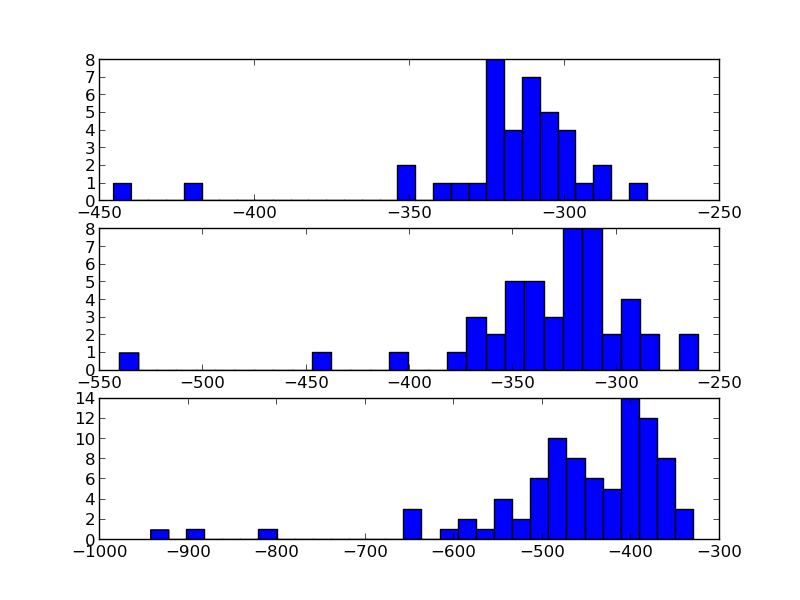
\includegraphics[trim= 0 0 0 0, clip=true, scale=0.7]{histograms.png}
    \caption{\small{\emph{figure 1}}}
  \end{minipage}
\end{figure}
\subsection*{subsection 1}
phrase 2.
\subsection*{subsection 2}
phrase 3.

\section*{Second Section}
phrase 4.
\subsection*{subsection 3}
phrase 5.
\subsection*{subsection 4}
phrase 6.
\end{document}
